\subsection{Tuple At A Time}

On figure \ref{fig:R0} is shown an algebraic plan corresponding to a direct translation of the query pattern into SQL++ algebra, which we denote as the \emph{tuple-at-a-time} (TAAT) algebraic formulation. This plan is the plan which semi-structured databases would generate initially, before any algebraic rewriting optimizations are performed. For this reason, we also call this formulation the initial plan. The plan on the left side of the figure corresponds to the translation of the outer query (denoted \emph{outer plan}), while the plan (denoted as $P$) in the dashed-lined box is the translation of the inner query (denoted as \emph{inner plan}). 

% \jules{Ensure that path variables are not used in algebra}

% Describe the outer query expression
\textbf{Outer Plan} The expression $E$ of the outer plan corresponds to the algebraic translation of the outer query SQL clauses below and including the \texttt{FROM} clauses, while the expression $G$ is the translation of the \texttt{SELECT} clause items other than the inner query. The apply plan operator $\alpha$ is correlated by variables $c_1, \dots, c_n$ while $z_1, \dots, z_{q'}$ are those variables produced by $E$ which are required by operators in $G$.

% Describe the inner query expression
\eat{
\textbf{Inner Plan} Within the inner plan (denoted as $P(c_1, \dots, c_n$), the translation of the \texttt{FROM} clause is shown on table \ref{table:taat-from}. It is defined recursively, where the value of $F(c_1, \dots, c_n)$ is translated into either: 1) a stored collection $R$, 2) a \texttt{FROM} item expression corresponding to the translation of a subquery (which recursively can have the $P$ normal form)correlated by attributes in $C_{subquery}$, itself a subset of $\{c_1, \dots, c_n\}$ 3) any kind of join ($\crossproduct$, $\innerjoin$, $\fullouterjoin$, $\leftouterjoin$, $\rightouterjoin$, etc.) between two \texttt{FROM} item expressions $F_{left}$, $F_{right}$ correlated by attributes in $C_{left}$, $C_{right}$, respectively. Note that any of $C_{subquery}, C_{left}, C_{right}$ could be empty, in which case the \texttt{FROM} item would be uncorrelated.
\begin{table}[]
\centering
\caption{Value of $F(c_1, \dots, c_n)$ \label{table:taat-from}}
\begin{tabular}{C{3cm} C{4cm}}
1) Stored collection   & $Scan_{R \mapsto r}$  \\
2) Subquery  & $F_{subquery}(C_{subquery})$  \\
3) Join between two \texttt{FROM} item & $Join_c(F_{left}(C_{left}),F_{right}(C_{right})$ \\
\end{tabular}
\end{table}
}

\textbf{Inner Plan} Within the inner plan (denoted as $P$), the value of $F(c_1, \dots, c_n)$ corresponds to the translation of the \texttt{FROM} clause expression $\hat{F}(c_1, \dots, c_n)$.  Next, operators $\sigma_w$, $\groupby_{g_1,\ldots,g_i; a_1(.) \mapsto A_1, \ldots, a_m(.) \mapsto A_m}$, $\sigma_h$, $\tau_{o_1, \dots, o_j}$, $\lambda_l$ correspond to the algebraic translation of the query pattern's \texttt{WHERE}, \texttt{GROUP BY}, \texttt{HAVING}, \texttt{ORDER BY} and \texttt{LIMIT} clauses, respectively. Finally, operators $\partitionby_{x_1^1,\dots,x_{n1}^1; oc^1; w^1(.) \mapsto W^1}$, $\dots$, $\partitionby_{x_1^l,\dots,x_{nl}^l; oc^l; w^l(.) \mapsto W^l}$, $\alpha_{P_1 \mapsto N_1}, \dots, \alpha_{P_k \mapsto N_k}$ correspond to the \texttt{PARTITION BY} statements and subqueries present in the \texttt{SELECT} clause.

\jules{@Yannis: one tricky thing to notice here is the position of the Apply plan ($\alpha$) operators, which reflect here the possible presence of nested queries in the input's \texttt{SELECT} clause. However, given we allow any arbitrary SQL++ expression in the \texttt{WHERE}, \texttt{GROUP BY}, etc clauses, we could, for example, have a subquery in the \texttt{WHERE} clause. Those would not be accounted for in this translation of the plan.}

\begin{figure}[h]
\centering
\caption{Tuple-At-A-Time Formulation (TAAT) \label{fig:R0}}
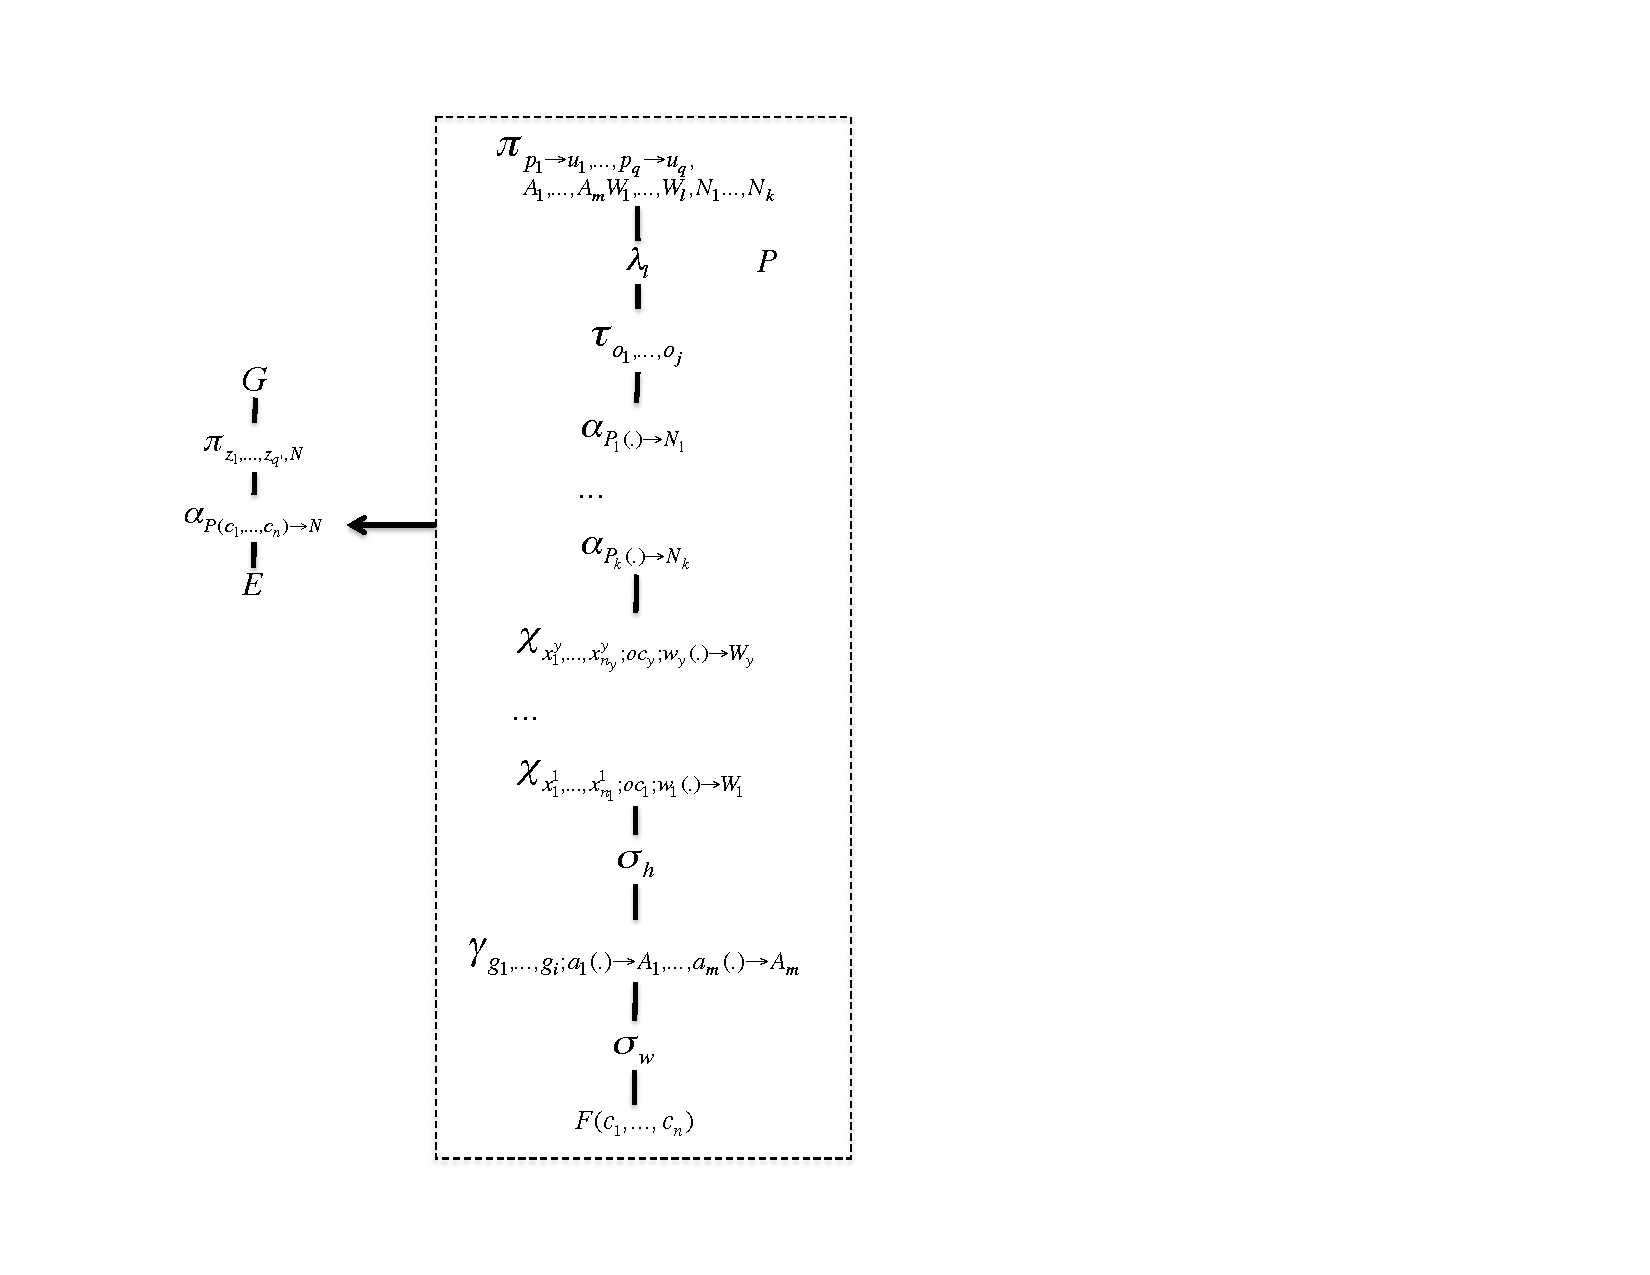
\includegraphics[width=0.85 \linewidth]{images/R0.pdf}
\end{figure}

The tuple-at-a-time formulation shown above constitutes only one way to formulate the query pattern. In particular, it evaluates the inner plan $P$ once for every binding tuple in the output of $E$. We present next two alternative algebraic formulations which evaluate the inner query for every binding tuple at the same time, which we denote as a set-at-a-time execution. We distinguish the \emph{normalized} and \emph{denormalized} set-at-a-time executions.

\subsection{Normalized Set-at-a-time \label{sec:NSAAT}}

The normalized set-at-a-time (NSAAT) formulation of the query pattern is shown on the figures \ref{fig:R2} and \ref{fig:from-items}. We obtain this formulation by rewriting the tuple-at-a-time formulation. Instead of evaluating a very similar (only differing by the value of the correlated attributes) inner query for each tuple in the output of $E$, it will (i) introduce a cross product between $E$ and the leaves of the inner plan $P(c_1, \dots, c_n)$ (ii) execute the inner plan only once on the output of this cross product (iii) group the tuples in the output of this inner plan according to the tuple of $E$ they correspond to (iv) create the nested collections using the \texttt{NEST()} aggregate function (v) join back with the original $E$ to preserve cardinality. Thus, the normalized set-at-a-time formulation replaces the tuple-at-a-time nesting operator $\alpha$ with a set-at-a-time nesting operator $\gamma_{\texttt{NEST}}$. The details of the rewriting are as follows:

\begin{figure}[h]
\centering
\caption{Normalized Set-At-At-Time Formulation (NSAAT) \label{fig:R2}}
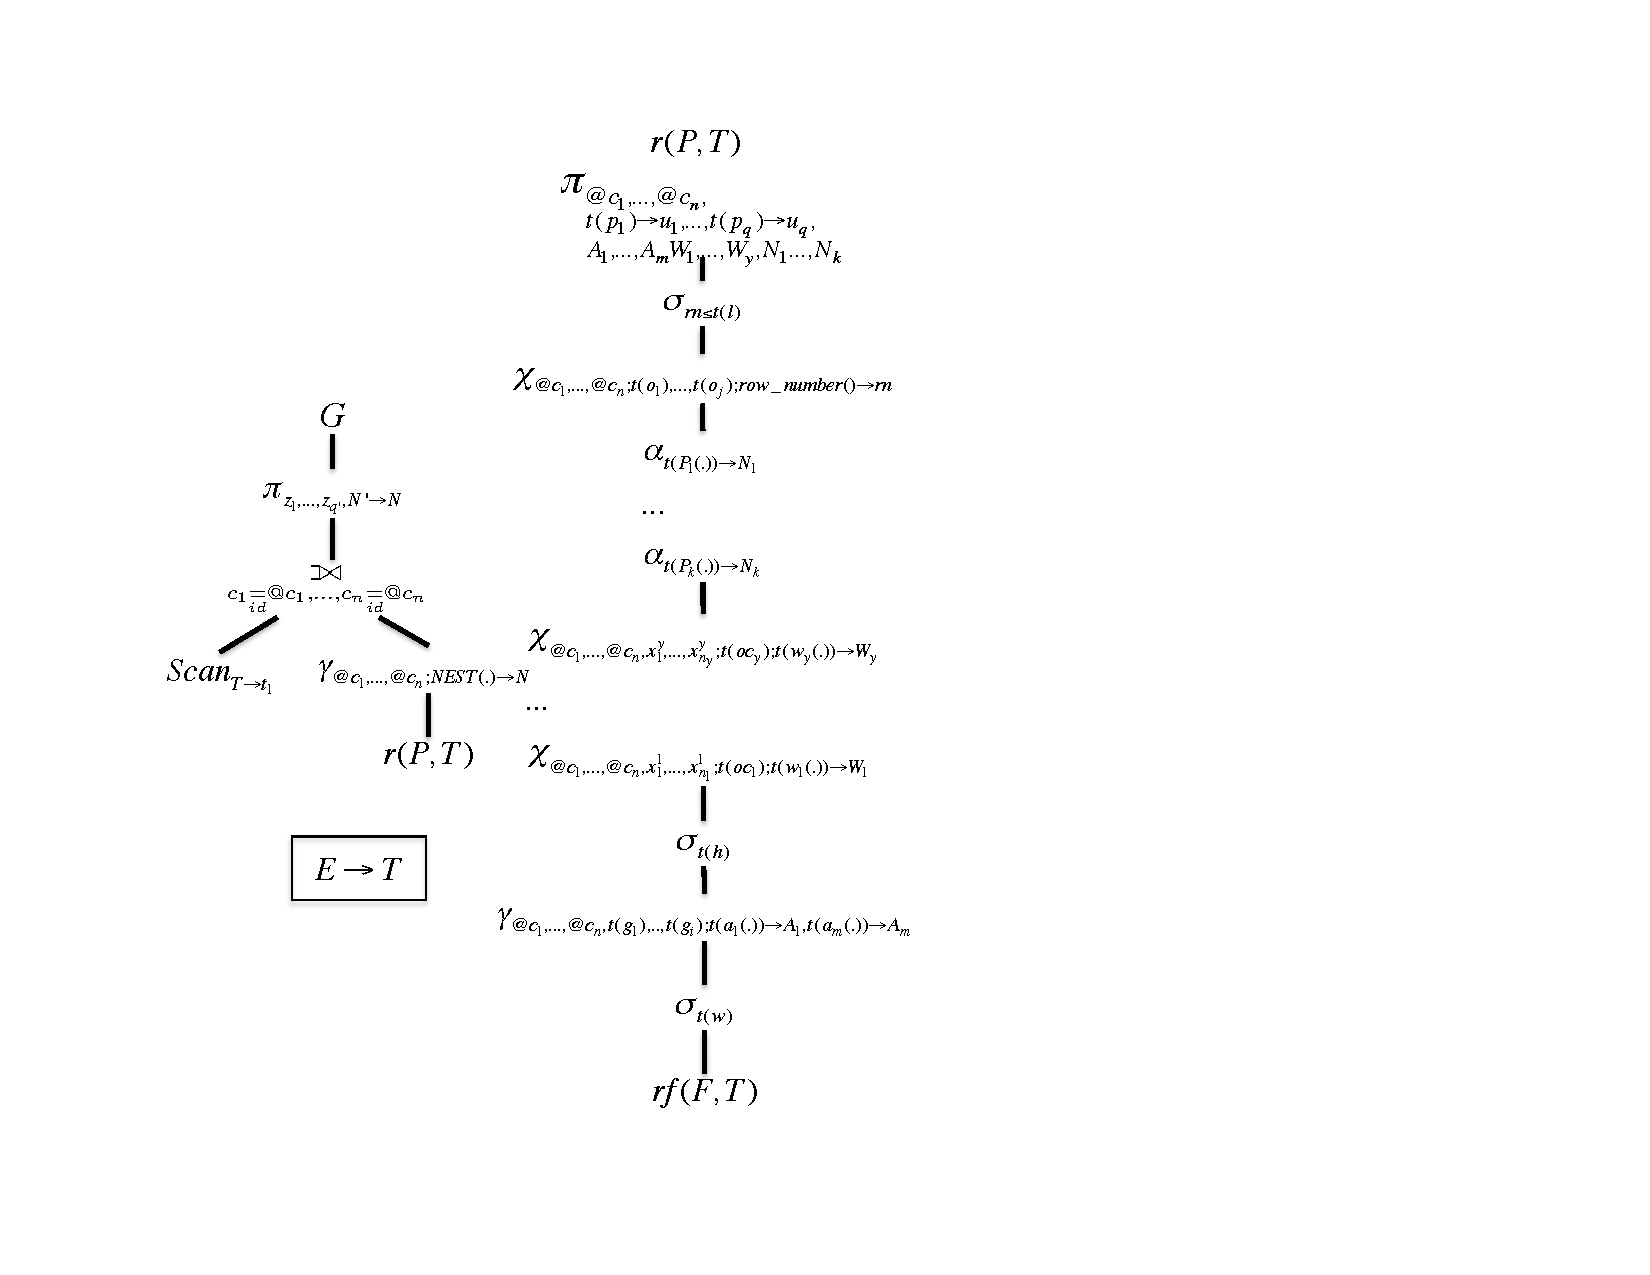
\includegraphics[width=\linewidth]{images/R2.pdf}
\end{figure}

% Outer Plan
\textbf{Outer Plan} The rewriting of the outer plan is shown on figure \ref{fig:R2}. The output of $E$ is assigned to a temporary table $T$. The plan $P$ is rewritten to $r(P,T)$ (as explained below). The result of this rewritten plan goes to a $\gamma_{\texttt{NEST(.)}}$ operator that groups according to the correlated attributes $c_1, \dots, c_n$ and nests all the binding tuples with the same correlated values. As we will see next, the group of binding tuples nested with a given set of correlated values $v_{c_1}, \dots, v_{c_n}$ corresponds exactly to those bindings which would be outputted by the original $P$ if parameterized with values  $v_{c_1}, \dots, v_{c_n}$. Next, a $\leftouterjoin$ operator joins this back with the original $T$ and a final $\pi$ operator ensures that the extra attributes created by the outer join are projected out. $\pi$ also replaces the \texttt{null} values introduced by the outer join with empty collections (in the figure, $N'$ stands for the translation of the SQL++ statement \texttt{CASE WHEN N IS NULL THEN [] ELSE N}). Note that if the original inner plan is a total aggregation query, the $\gamma^T_{a_1(.) \rightarrow A_1, \dots, a_m(.) \rightarrow A_m}$ is rewritten into $\gamma^T_{c_1, \dots, c_n; a_1(.) \rightarrow A_1, \dots, a_m(.) \rightarrow A_m}$. In this case, the top $\pi$ operator replaces \texttt{null} $N$ bindings with a collection containing a single tuple with default values for each total aggregate function in the original query. \jules{The approach above could be problematic because it does not distinguish between the \texttt{null}s created by the outer join from the \texttt{null}s pre-existing on the right hand side. This is not a problem here because all binding tuples from the right hand side will have a non-null \texttt{N}}.

\begin{figure}[h]
\centering
\caption{\texttt{FROM} clause rewriting \label{fig:from-items}}
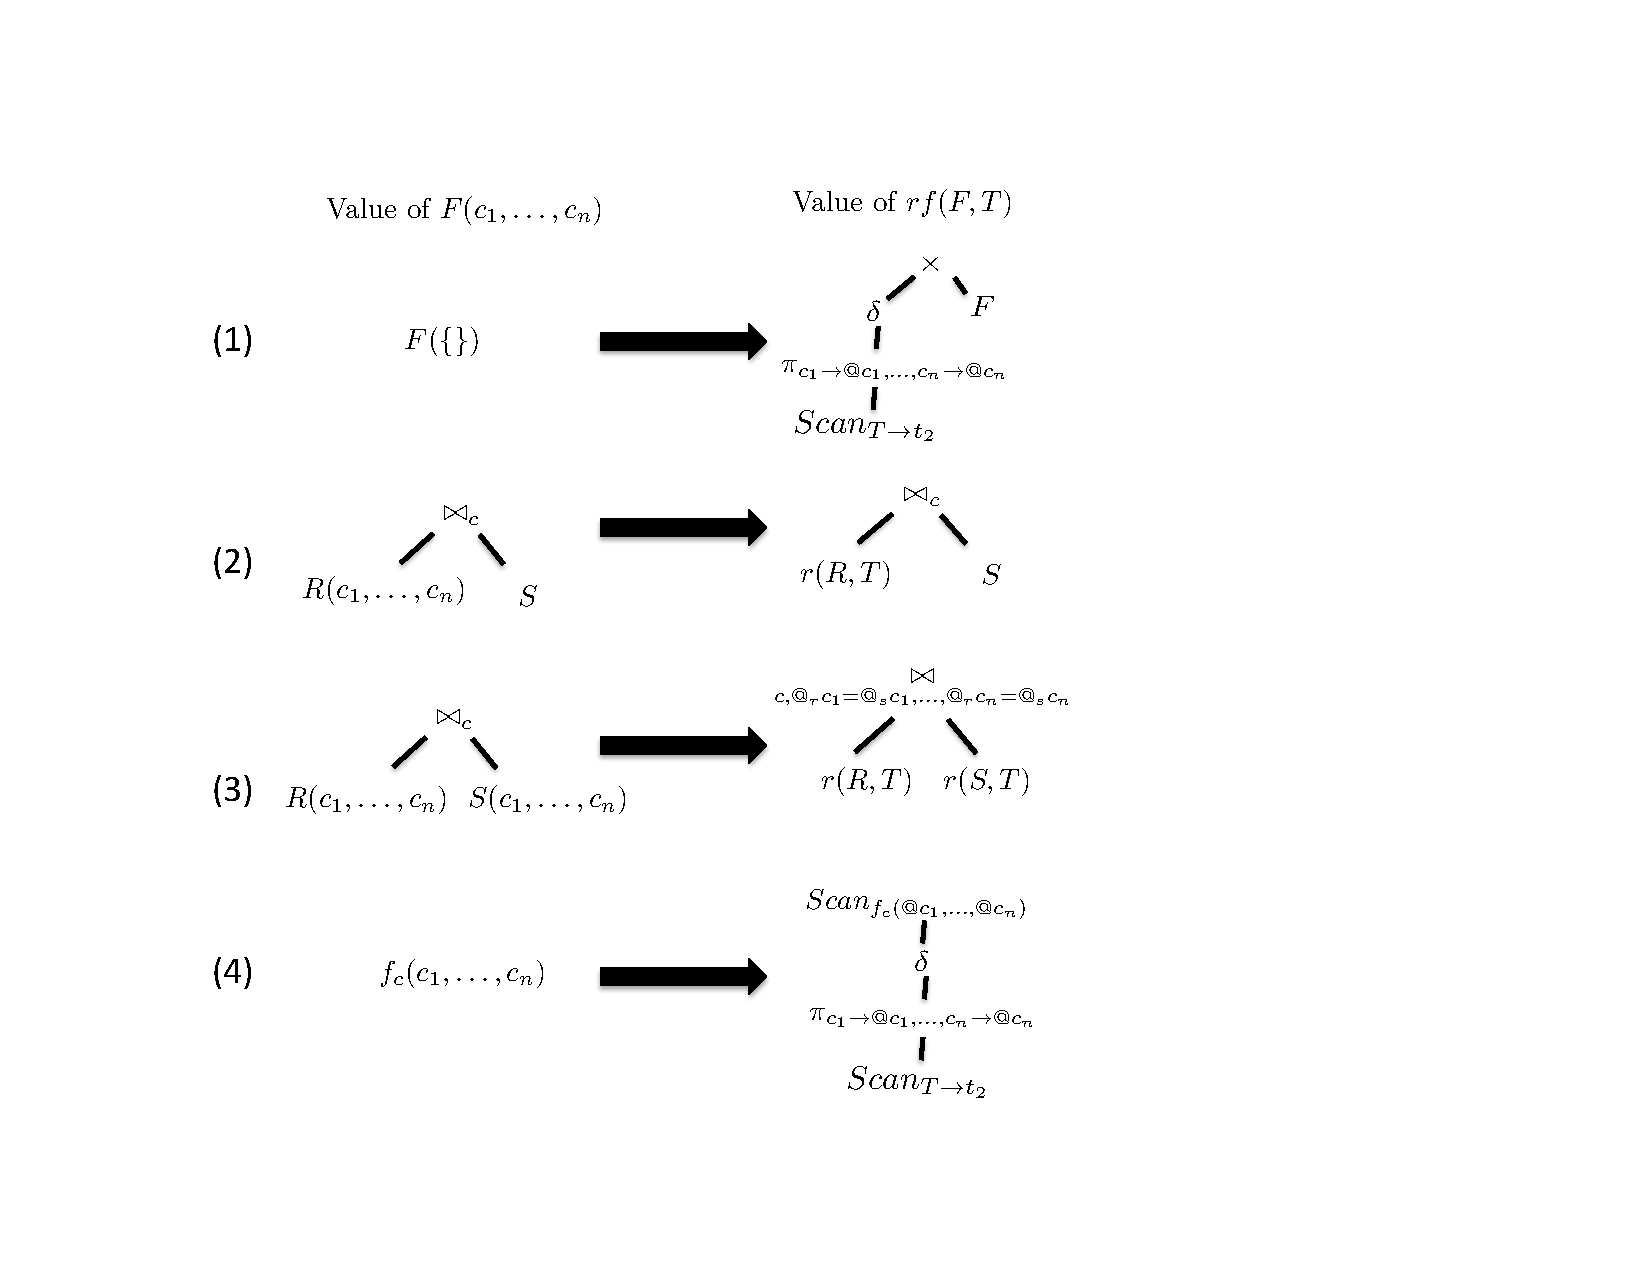
\includegraphics[width=\linewidth]{images/F_RF.pdf}
\end{figure}

We next describe how to rewrite the inner plan's \texttt{FROM} clause (figure \ref{fig:from-items}). The rewriting $r(P,T)$ of the nested plan $P$ introduces a cross product between the distinct correlated attributes of $T$ an the leaves of $P$. This is done by rewriting $rf(F,T)$ of the \texttt{FROM} clause $F$ of $P$. The rewriting of $F$ requires a case analysis (for conciseness, we treat $A \times B$ in the initial plan as $A \innerjoin_{true} B$ and do not explain it further): i) If $F$ is not correlated, it is rewritten into a simple cross product between $F$ and $\delta(\pi_{c_1, \dots, c_n}(T))$. A $\pi$ operator keeps only the correlated attributes $c_1, \dots, c_n$ renamed into $@c_1, \dots, @c_n$ (case 1 of figure \ref{fig:from-items}). ii) If $F$ is one correlated subquery $R(c_1, \dots, c_n)$, it is recursively rewritten into $r(R,T)$ (not shown in figure). iii) if $F$ is a join between two \texttt{FROM} items, but only one is correlated $R(c_1, \dots, c_n)$, then only $R$ is recursively rewritten into $r(R,T)$ (if it is a subquery) or $rf(R,T)$ (if it is a join).  iv) If $F$ is a join between two correlated branches $R(c_1,\dots,c_n)$ and $S(c_1,\dots,c_n)$, both are recursively rewritten to  $r(R,T)$ / $rf(R,T)$ and $r(S,T)$ / $rf(S,T)$ if they are subqueries/joins respectively. Moreover, the join condition $c$ is modified to enforce that the bindings outputted by the join correspond to the same values of correlated attributes on both sides (case 3 of figure \ref{fig:from-items}, $@$ symbols have additional subscripts to distinguish the renamings on the left and right hand side ).  v) If $F$ is a correlated expression (e.g. a path starting from a correlated variable and evaluating to a collection), it is rewritten into an unnesting Scan of $t(f_c(c_1, \dots, c_n))$ on top of $\delta(\pi_{c_1, \dots, c_n}(T))$. vi) Finally, if a join condition in $F$ is correlated, the rewriting corresponds to the case when both branches are correlated and the join condition is rewritten into $t(c)$ (not shown in the figure). Notice that the value of $rf(F,T)$ in cases (1) and (4) from figure \ref{fig:from-items}. The duplicate elimination is only required if there may be duplicate correlate attributes in the input.  In the case where the set of correlated attributes includes a key to the output of expression $E$ ($key(E) \subseteq \{c_1, \dots, c_n\}$), the $\delta$ operator can be eliminated.

% Inner Query
\textbf{Inner Plan} The rewriting of the inner plan $P$ is shown on figure \ref{fig:r2}. If $X$ is or an expression of plan $P$ correlated by attributes $c_1, \dots, c_n$, we denote $t(X)$ the same expression $X$ in which the attributes $c_1, \dots, c_n$ are substituted with variables $@c_1, \dots, @c_n$. i) The top $\pi$ operator of $P$ is modified to also output the attributes $@c_1, \dots, @c_n$ necessary for the $\gamma_{\texttt{NEST}(.)}$ and $\leftouterjoin$ operators above. iii) The nested plans $P_1, \dots, P_k$ of eventual $\alpha$ operators in $P$ are rewritten to $t(P_1), \dots, t(P_k)$. iv) The eventual $\tau$ and $\lambda$ operators are replaced with two other operators: on the one hand, a $\chi$ operator that groups according to $c_1, \dots, c_n$, orders according to the $t(o_1), \dots, t(o_j)$, then computes the row number of each tuple in its partition. The row number can then be used with a $\sigma$ operator to simulate the $\lambda$ (note that, depending on the implementation, if the $\gamma$ operator at the top of the rewritten plan breaks the ordering between the binding tuples coming from the $\chi$, the \texttt{NEST} function will have to sort again the tuples in each nested collection according to the row number). v) The grouping attributes of the eventual $\chi$ operators of $P$ are modified to also group by $@c_1, \dots, @c_n$. vi) The \texttt{HAVING} clause condition $h$ is rewritten to $t(h)$. vii) The grouping attributes of the eventual $\gamma$ operator of $P$ are modified to also group by $@c_1, \dots, @c_n$. viii) The \texttt{WHERE} condition $w$ is rewritten to $t(w)$.

\eat{
\begin{table}[]
\centering
\caption{Value of $rf(F,T)$ \label{table:saat-from}}
\begin{tabular}{C{3cm} C{3.5cm}}
1) Stored collection   & $\times(\delta(\pi_{c_1, \dots, c_n}(Scan{T \mapsto t_2})), Scan_{R \mapsto r})$  \\
2) Subquery  & $F_{subquery}(C_{subquery})$  \\
3) Join between two \texttt{FROM} item & $Join_c(F_{left}(C_{left}),F_{right}(C_{right})$ \\
\end{tabular}
\end{table}
}

\subsection{Denormalized Set-at-a-time}

The denormalized-set-at-a-time (DSAAT) formulation of the query pattern is shown on figure \ref{fig:R4}. We also describe this pattern rewriting of the TAAT formulation. 

% Where clause 

% Investigating further restrictions on the denormalized set-at-a-time.



% Restriction
$E$ has to be a set. It can't just be a 

\begin{figure}[h]
\label{fig:R4}
\centering
\caption{Denormalized Set-At-At-Time Formulation (DSAAT)}
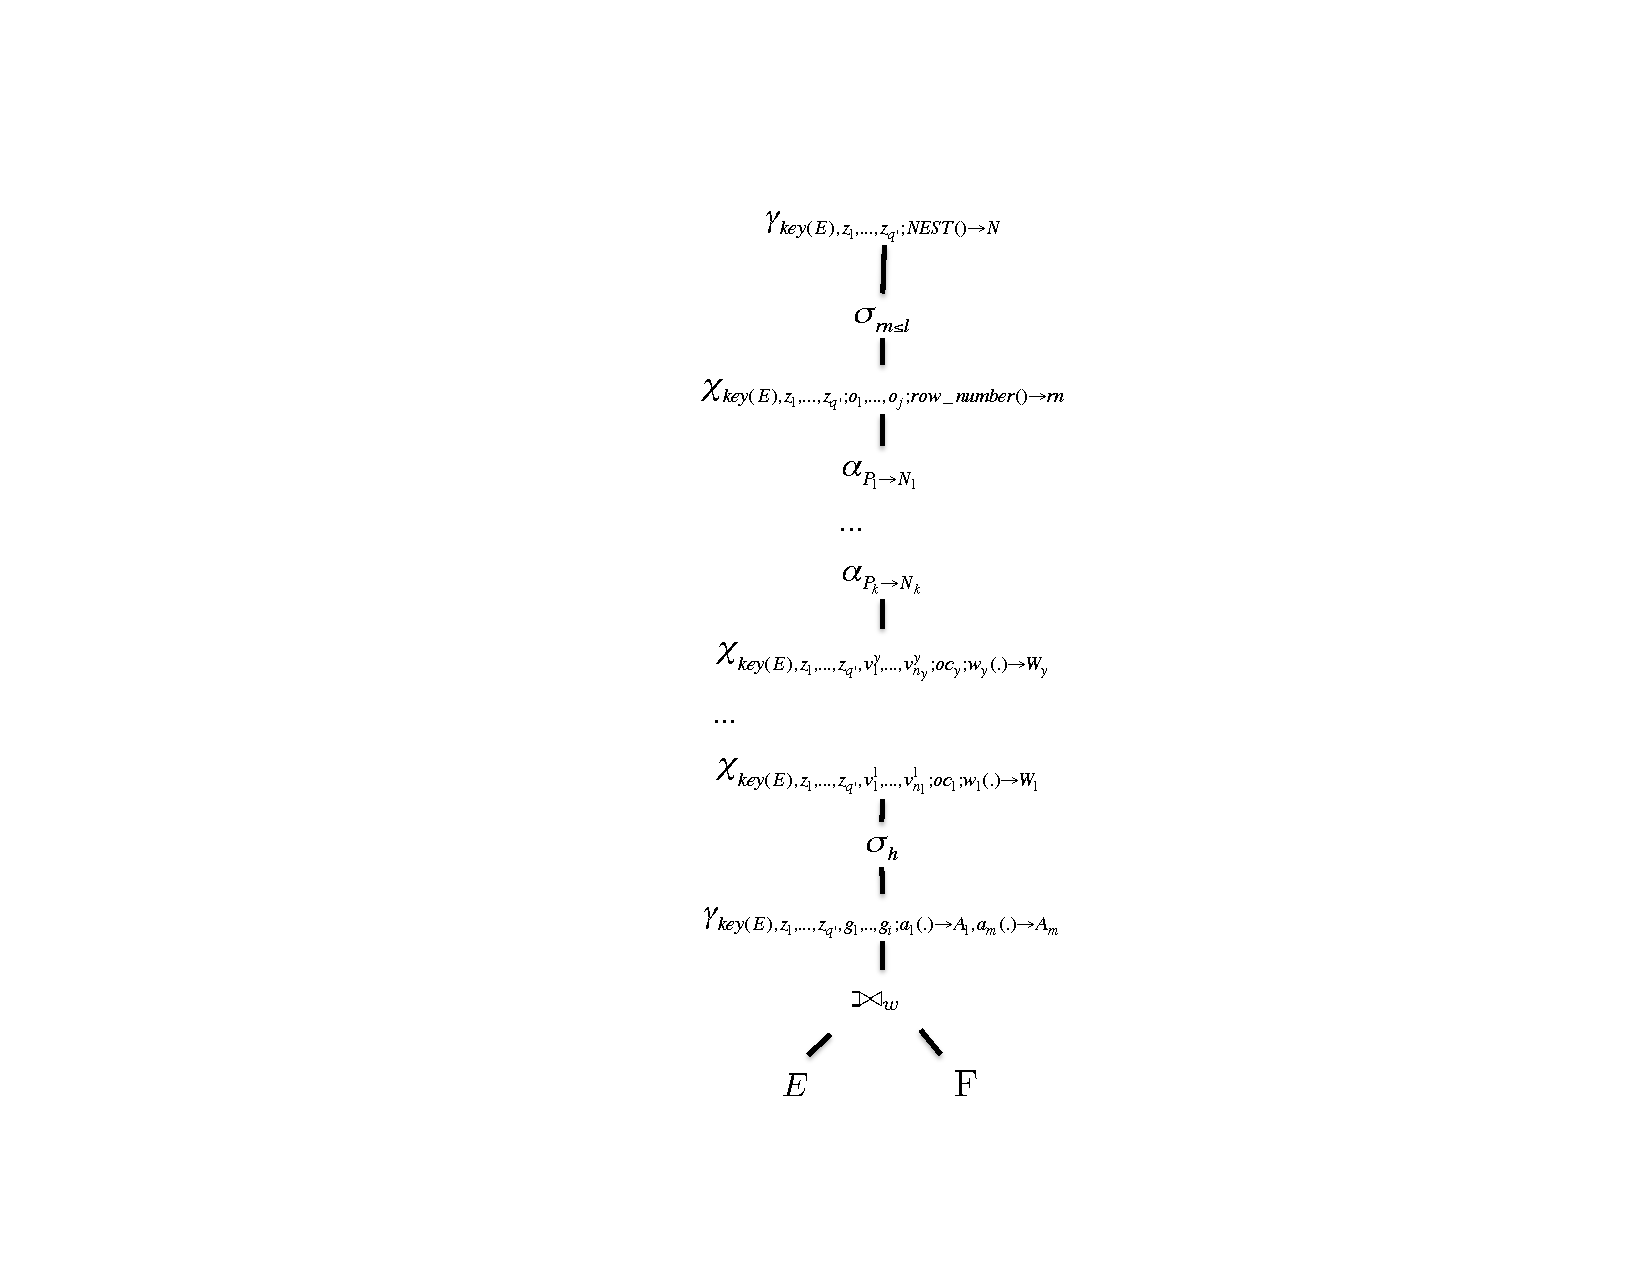
\includegraphics[width=0.65 \linewidth]{images/R4.pdf}
\end{figure}